\documentclass[12pt]{article}
\usepackage{color}
%\usepackage{portland}
\usepackage{jasa,helvetica}
\input vu.sty
\input /home/jba/.texinputs/mac.sty
\usepackage{psfig}
\usepackage{headerfooter}

%%%%% remove to make HTML %%%%%
%\usepackage{vu,mac}
%%tth: \usepackage[dvips]{graphics}
%%%%% use to make HTML: l2h Talk -e2 %%%%
%%tth: \input /home/jba/.texinputs/vu.sty
%%tth: \input /home/jba/.texinputs/mac.sty
%%tth: \renewcommand{\resizebox}[3]{#3}{}{}
%%tth: \newcommand{\Title}[1]{\begin{center} \huge #1 \end{center}}
%%tth: \newcommand{\Author}[1]{\begin{center} \Large #1 \end{center}}

\pagestyle{myheadings}
%\pagestyle{empty}
\pageheader{\it Sendai -- July 29, 1999} {\thepage} {Tectorial filtering, 2TS, USM}


\marginparwidth 0.85in
\setlength {\textwidth} {6.1 in} \setlength {\oddsidemargin} {2.5 mm}
\setlength {\textheight} {8.75 in} \setlength {\topmargin} {-5 mm}

\renewcommand{\Marginpar}[1]{}
\newcommand{\JND}{\mbox{\scriptsize JND}}
\newcommand{\citeay}[1]{\cite{#1}}

\begin{document}
	%\landscape
\Title
{ Is tectorial membrane filtering required to explain two-tone
suppression and the upward spread of masking?  }
\Author{J. B. Allen and Deep Sen\\
AT\&T Labs--Research\\
Florham Park, NJ 07932-0971}

\vspace{\fill}
 \flushleft{\tiny /doc/papers/Sendai.99/Talk.tex
\hspace{.5cm}\today}

%%%%%%%%%%%%%%%%%%%%%%%%%%%%
%%   Start of material    %% 
%%%%%%%%%%%%%%%%%%%%%%%%%%%%

\newpage
\Heading{The place to frequency map}
\I{The {\blue cochlear map} describes the location of the frequency
maximum of the tuning curve along the cochlear partition}
\I{From basic theory $f_{cf} = \sqrt{K(x)/M}/2 \pi =f_{max}e^{-ax}$}
        \begin{center}
\resizebox{ 0.6\textwidth }{!}{ 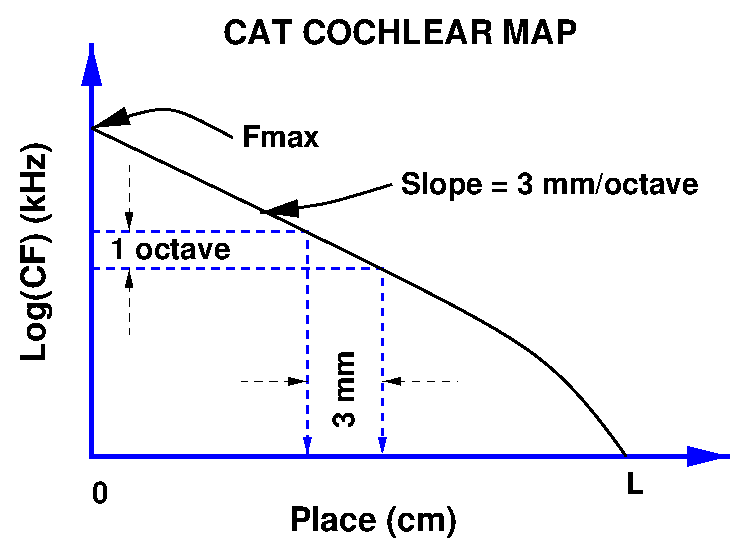
\includegraphics{figs/cmap.eps} }
        \end{center}       

	\B

\I{The {\blue constant} $a = -0.231\;\;(mm^{-1})$ for the Cat
may be computed from the slope (3 mm/oct)
\[
2 = e^{-a \; 3} \rightarrow a = -\log(2)/3 \;\; (mm^{-1})
\]
}
	\E
\E

\newpage
\Heading{Transmission line model}
\I{The 1D cochlear model}
\vspace{.2cm}
        \begin{center}
\resizebox{ 0.5\textwidth }{!}{ 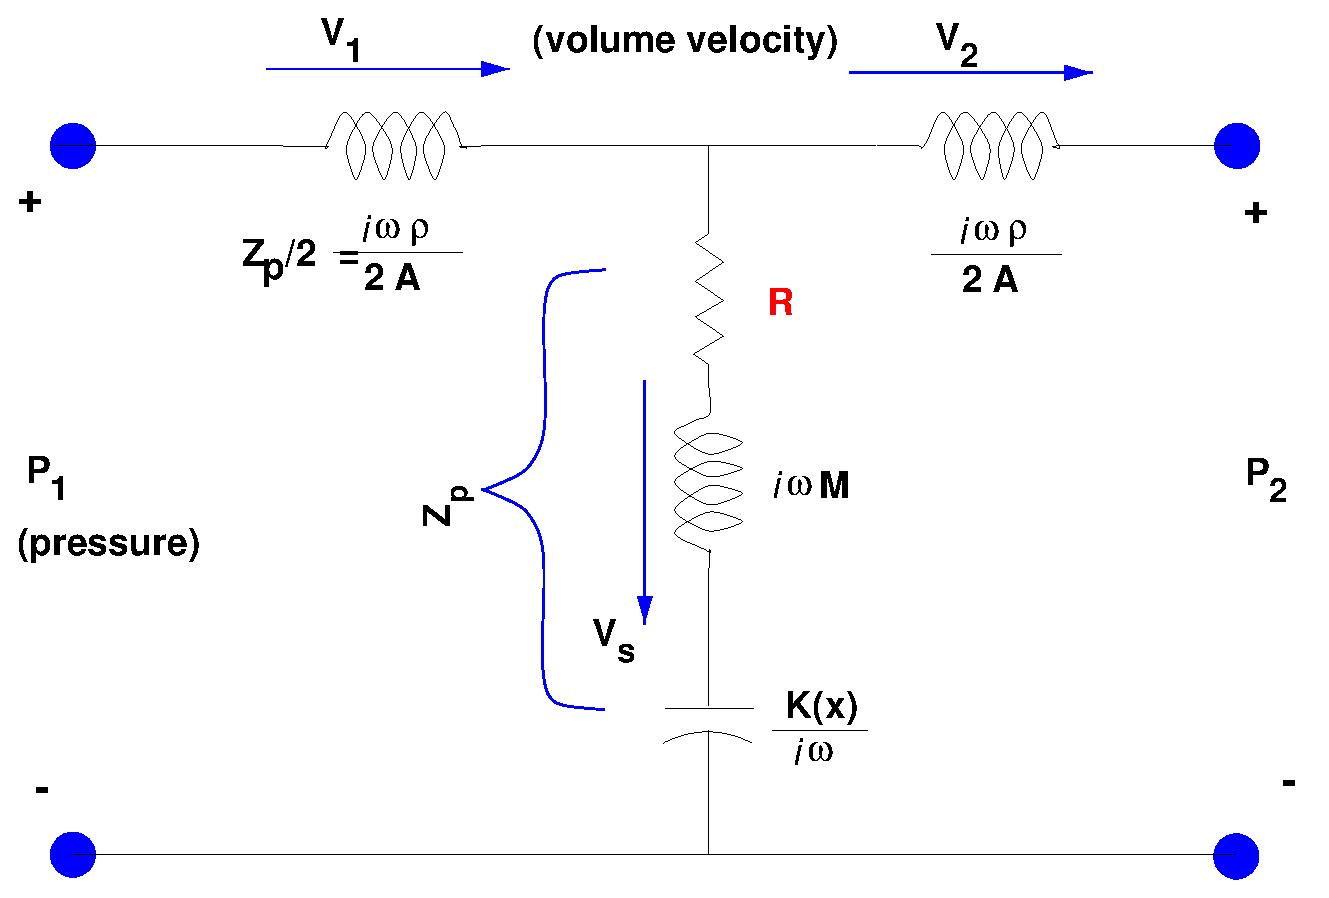
\includegraphics{figs/tline.eps} }
        \end{center}       

\I{The scala impedance: $Z_p = i \omega \rho / A$ }

\I{The cochlear partition impedance:
	\[
Z_{p}(x,\omega) = {K_0 e^{-2ax}}/{i \omega} + R_0 + i \omega M
	\]\\
	}
        \begin{center}
\resizebox{ 0.6\textwidth }{!}{ 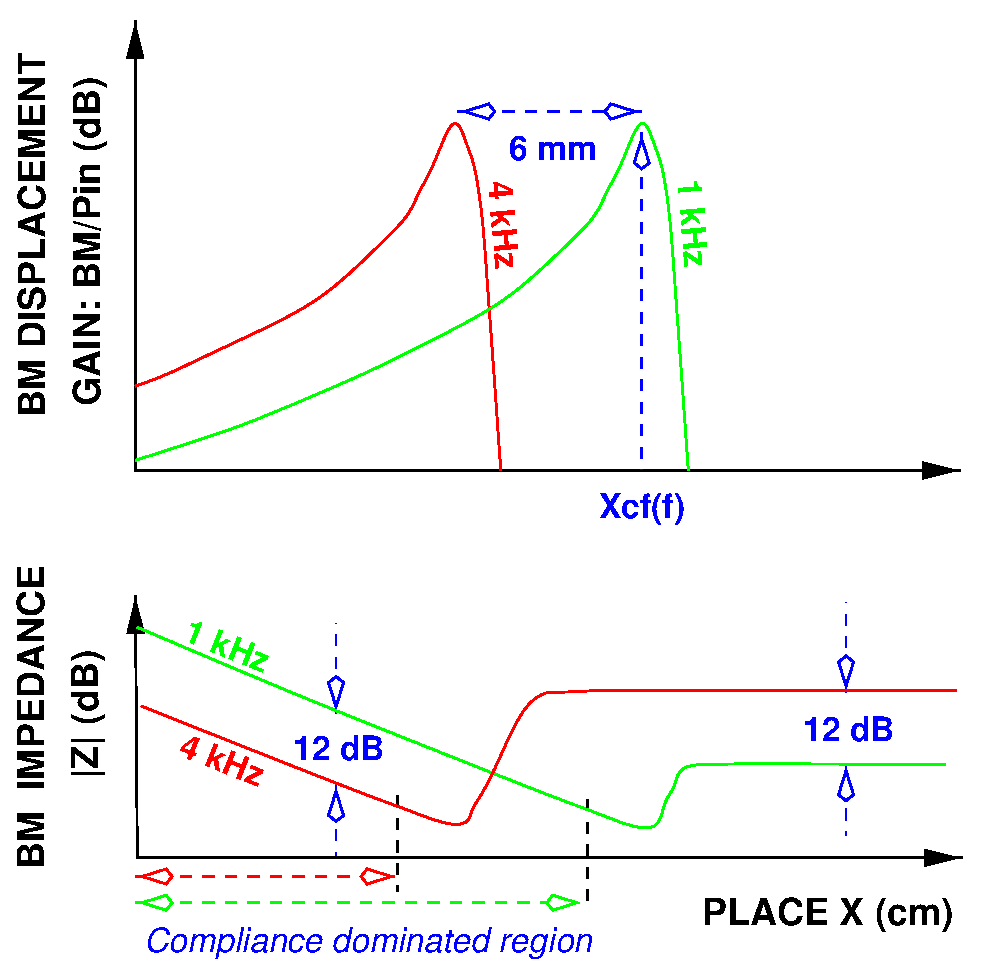
\includegraphics{figs/imped.eps} }
        \end{center}       
\E

\newpage
\Heading{Neural excitation pattern}
\I{Neural tuning curves along with the cochlear map allow us to
estimate {\blue neural excitation patterns} }

        \begin{center}
\resizebox{ 0.95\textwidth }{!}{ \includegraphics{figs/eplftc.eps} }
        \end{center}       

\I{These {\blue frequency domain} data were transformed to
the {\blue place domain} using Liberman's cochlear map 
\[ f_{cf} = 456 \left [ 10^{2.1(1-x/L)} -0.8 \right ] \]
	}
        \begin{center}
\resizebox{1.05\textwidth }{!}{ 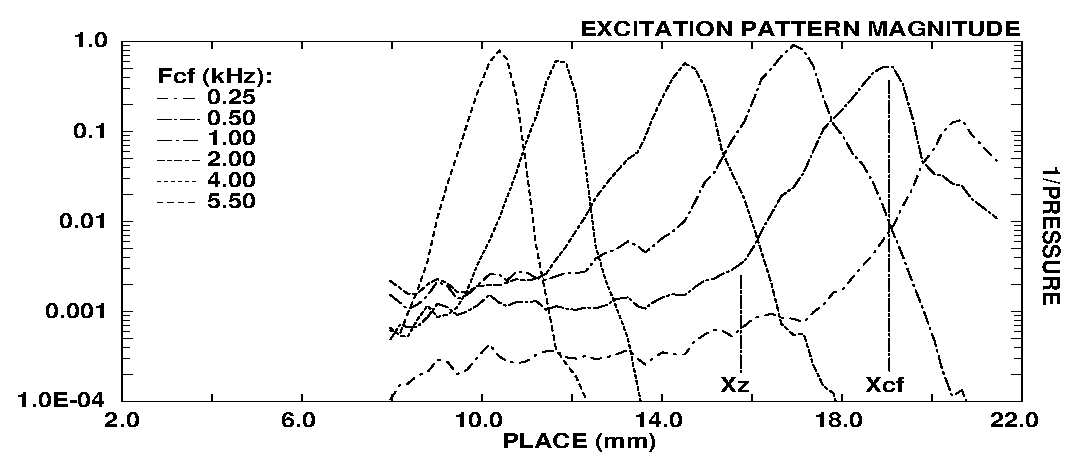
\includegraphics{figs/ep.eps} }
        \end{center}       
\E

\newpage
\Heading{Stiffness dominated tail region}
\I{ For each pure tone stimulus, the partition impedance is
compliance dominated from the stapes to $X_z(f_{cf})$
(i.e., a few mm basal to the CF)
\[
{\blue Z_{p}(x,\omega) \approx {K_0 e^{-2ax}}/{i \omega}}
\]
	}

        \begin{center}
\resizebox{ \textwidth }{!}{ 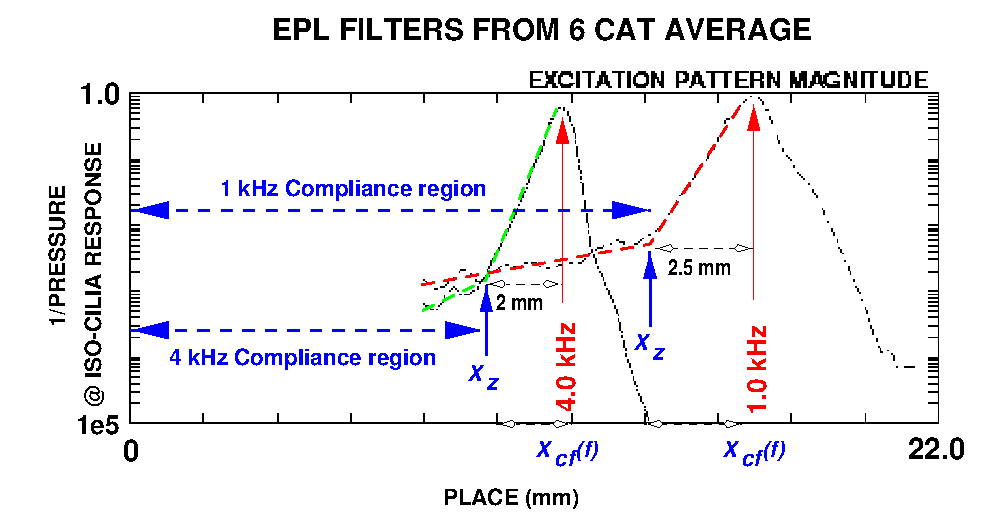
\includegraphics{figs/expat2.eps} }
        \end{center}       

\I{{\blue Hooke's Law} relates partition pressure $P(x)$
and displacement $D(x)$
\[
	P(x) = K_0 e^{-2ax} \; \; D(x)
\]\\
	}
\E

\newpage
\Heading{Cochlear Pressure for a tone}
\I{From the WKB solution method, the spatial pressure distribution
of a tone stimulus in the base of the cochlea is given by
	\begin{eqnarray*}
\frac{P(x,\omega)}{P(0,\omega)}
	&=&
\sqrt{\frac{Z_{char}(x)}{Z_{char}(0)}}
	\ \ e^{-i\omega \int _{\xi =0}^x d\xi/c(\xi) } \\
	&=&
		 e^{ -ax/2 }\ e^{ -i\omega \tau(x,\omega)}.
	\end{eqnarray*}
	}


\I{Conclusion: From Hooke's Law, since}
	\B
\I{The partition pressure magnitude {\red decays} as
	\[ |P(x)| \propto e^{-ax/2} \;\;\;(-1\ dB/mm) \] \\}
\I{{\blue It follows that:}
The partition displacement magnitude {\red increases}
as
\[ |D(x)| \propto e^{3ax/2} \;\;\; (+3\ dB/mm) \]\\}
	\E

\I{Since the inner haircell is a displacement detector above
about 1 kHz the cat the cilia (neural) response should grow
as {\blue 3 dB/mm}}
\E

\newpage
\Heading{Estimation of basal EP slope}
\I{Neural excitation pattern estimated from FTC
        \begin{center}
\resizebox{\textwidth }{!}{ 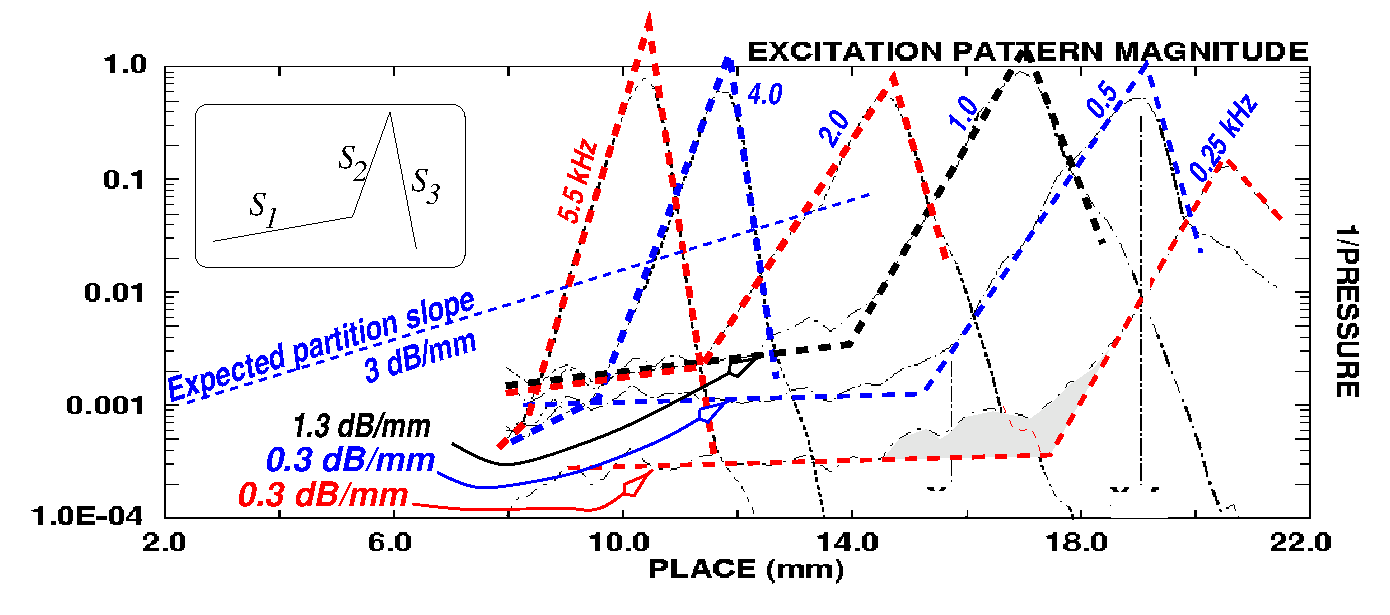
\includegraphics{figs/ep1.eps} }
        \end{center}       
	}
\I{Slopes $S_1$, $S_2$, and $S_3$ (\emph{dB/mm})
        \begin{center}
\begin{tabular}{c|ccc} \hline \hline
CF & $S_1$ & $S_2$ & $S_3$ \\ \hline
{\large \it kHz} &  & {\large \it SLOPE$^{\red *}$ (dB/mm)} & \\ \hline 
5.0 & {\blue **} &   32.7 &  -66.1  \\
4.0 & {\blue **} &   26.3 &  -69.3  \\
2.0 & {\blue  1.3} &   15.2 &  -34.5  \\
1.0 & {\blue  1.2} &   17.4 &  -25.6  \\
0.5 & {\blue  0.3} &   14.8 &  -34.5  \\
0.25 &{\blue  0.3} &   17.1 &  -11.0  \\ \hline
\end{tabular}
	\end{center}

{\red \large \ $*$ Mult by 3 mm/oct to convert to dB/oct}\\
{\blue \large \ $**$Not enough data.}

	}
\E

\newpage
\Heading{A natural solution to the transduction filter problem}
\I{I propose that the partition stiffness is dominated by the
tectorial membrane stiffness $K_t(x)$ }
        \begin{center}
%Started from /home/jba/doc/papers/NL-RTM.98/figs/model.fig
\resizebox{ 0.90\textwidth }{!}{ 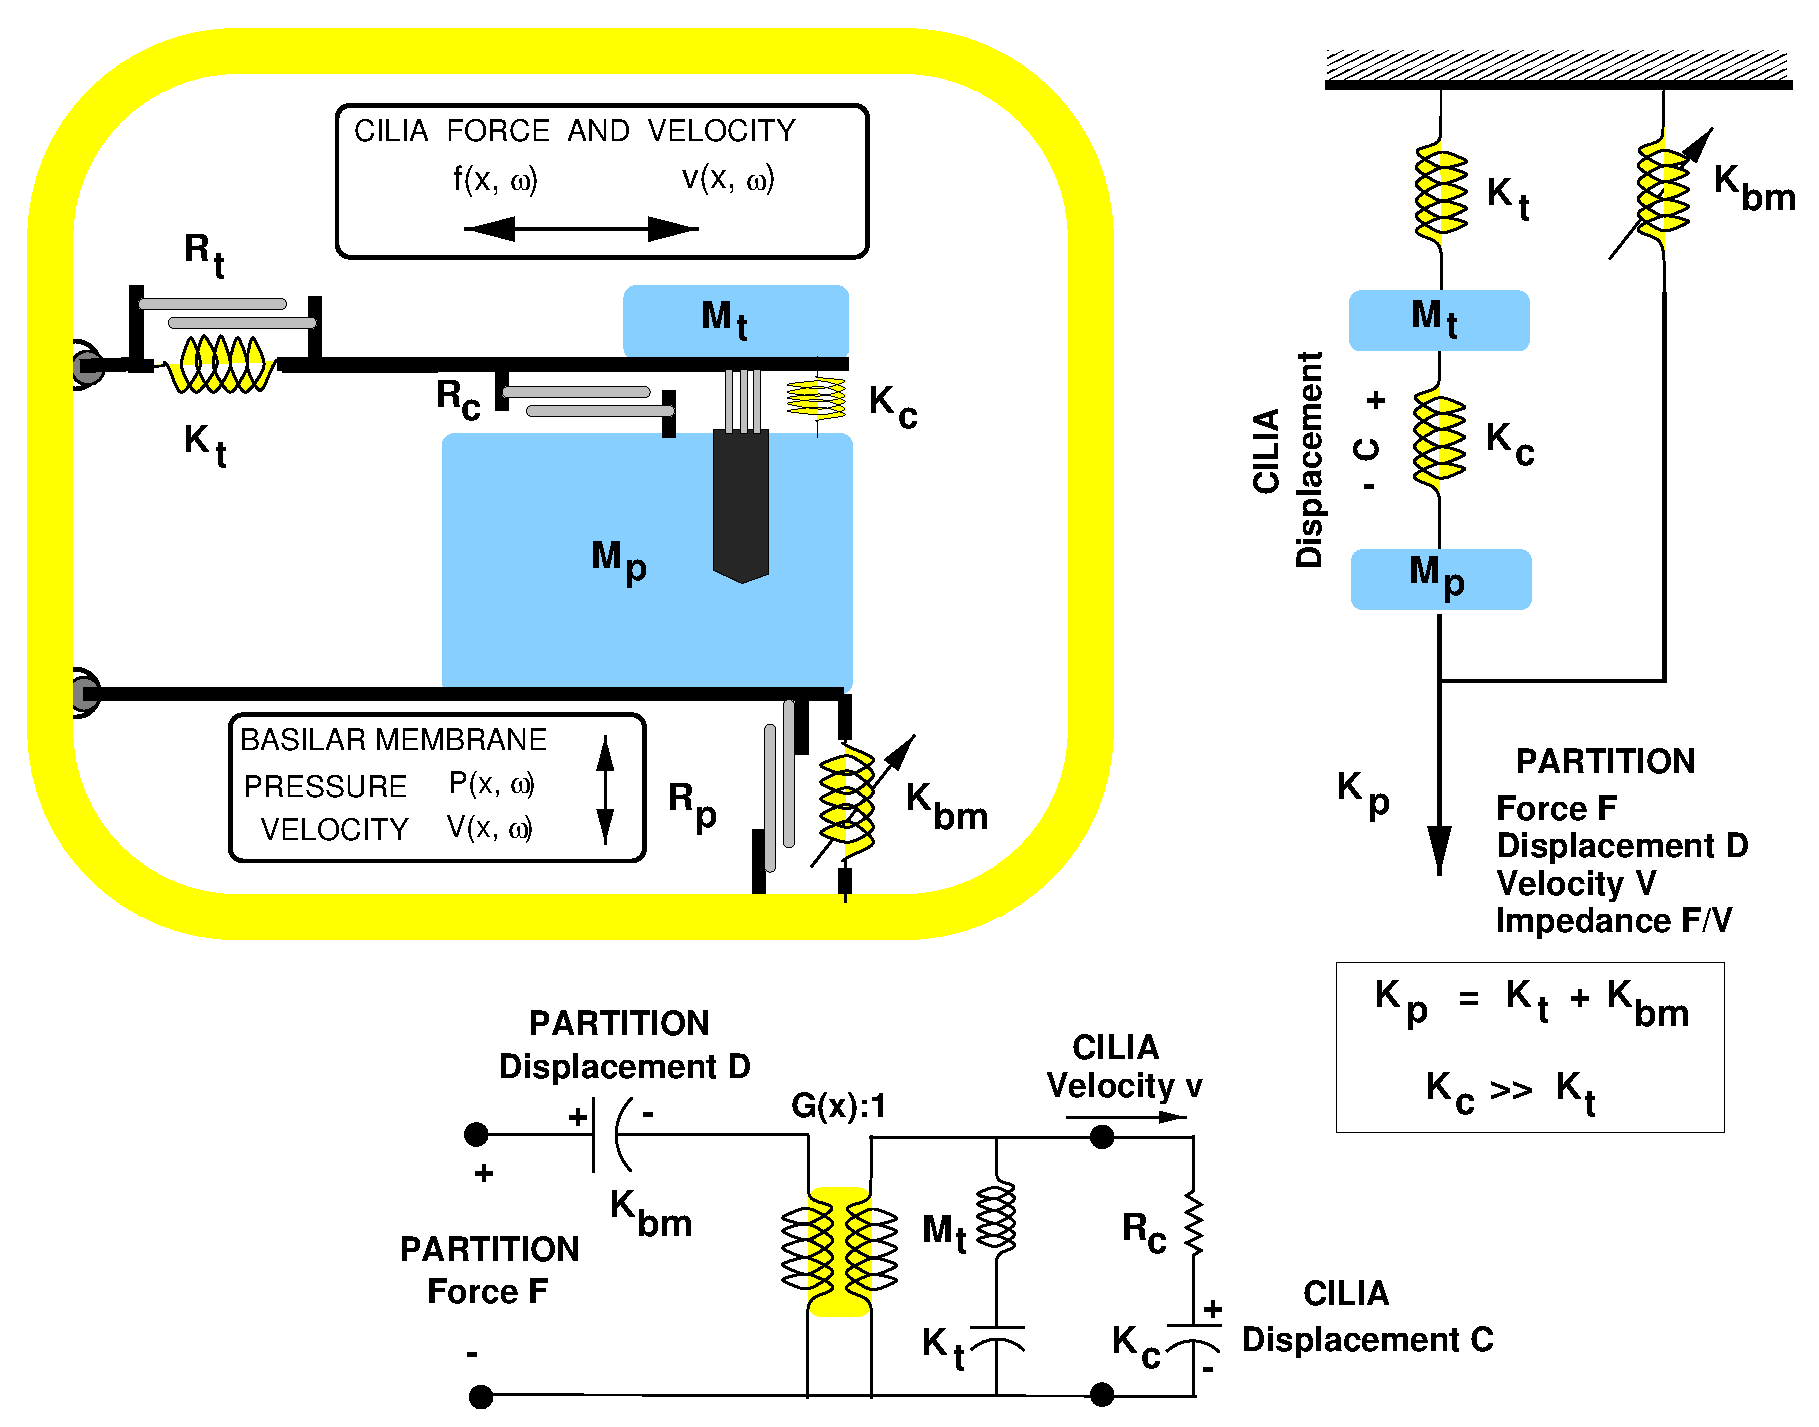
\includegraphics{figs/rectamodel.eps} }
        \end{center}       
\I{The partition impedance is:
	 $K_p = \frac{K_t K_c}{K_t + K_c} + K_{bm}$ }
	\B
\I{ Assume: $K_t/K_c \propto e^{-3ax/2}$ and $K_{bm} \approx K_t $ }
	\E
\I{This gives the two cochlear maps:
 \[
 f_{z}(x) \equiv \frac{1}{2 \pi}\sqrt{K_t/M_t} = f_{cf}(x)/\sqrt{2}
 \]
and the $e^{3ax/2}$ BM displacement growth is canceled
	\[
H \equiv \frac{C}{D} = K_t/K_c \approx e^{-3ax/2}
	\]
	}
\E

\newpage
\Heading{FINAL CONCLUSION:}
%\item[\cyan $\Rightarrow$] {\Large {\red
\I{{\red There must be a transduction filter} $H(x,f)$ to account
for the slope difference of 3 dB/mm for $D(x,f)$ and 0.3-1.3
dB/mm for the cilia EP $C(x,f)$ }
\I{ The basal slope must be small to match the threshold data
for the USM and 2TS }
\E
\vspace{1cm}
        \begin{center}
\resizebox{ 0.9\textwidth }{!}{ 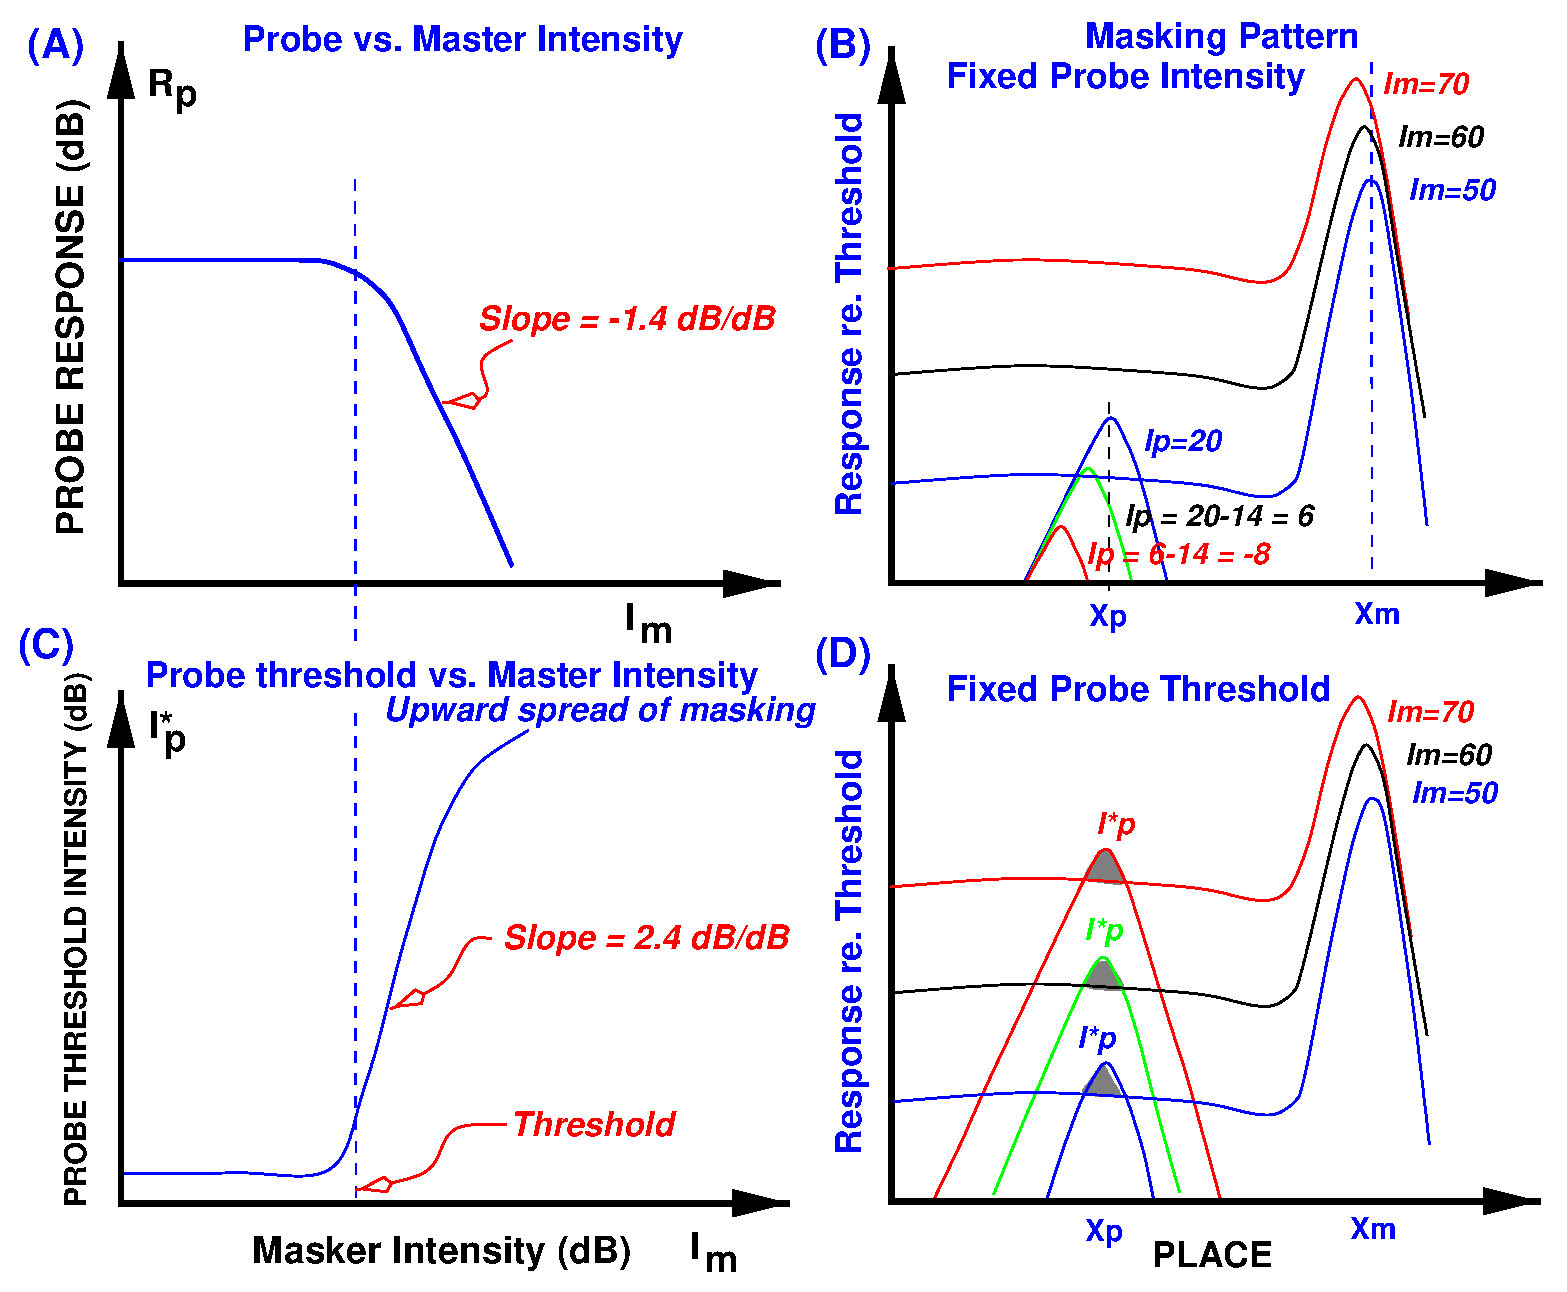
\includegraphics{figs/MaskedGain.eps} }
        \end{center}       

	\commentx{
\newpage
\bibliographystyle{jasa}
\bibliography{\bibpath/jnd,\bibpath/fletcher,\bibpath/books,%
\bibpath/loudness,\bibpath/allen,\bibpath/hcell,\bibpath/speech,%
\bibpath/model,\bibpath/ai}
	}

\end{document}
